\subsection{Bathymetry}
\label{sec: bathy}

	Survey data collected on October 1st was considered for the analysis. These data were measured via the CRAB and a Trimble Real Time Kinematic (RTK) GPS system. Elevation data from six cross-sections\footnote{we could potentially add an overhead plot of the transects}, perpendicular to the shoreline, spaced over a 100 meter portion of the beach were combined to create the 2-D surface shown below in Figure \ref{2-D Bath}. 
	
	\begin{figure}[h]
	\centering
	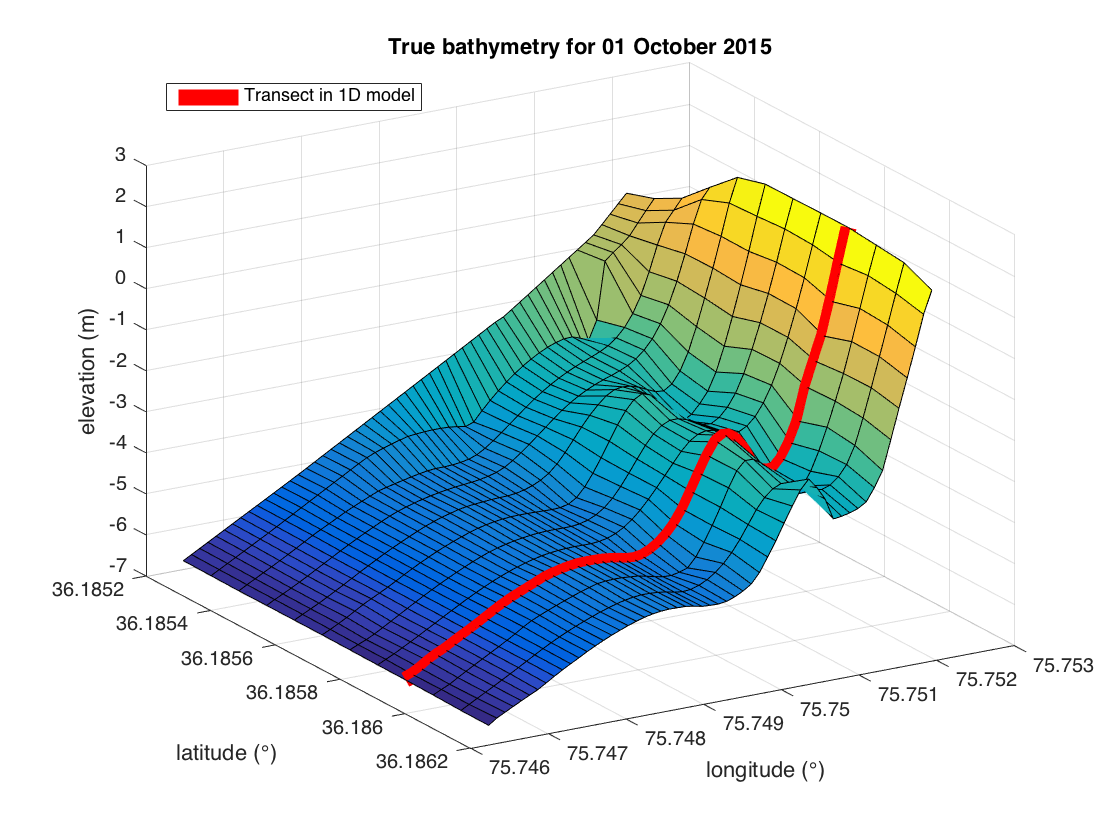
\includegraphics[width=.6\linewidth]{img/trueBath2D.png}
	\caption{2-D Bathymetry}
	\label{2-D Bath}
	\end{figure}